\documentclass{article}
\usepackage[utf8]{inputenc}
\usepackage{authblk}
\usepackage{amsmath}
\usepackage{amssymb}
\usepackage{graphicx}
\usepackage{physics}
\usepackage{float}
\usepackage{bm}
\usepackage{caption}
\usepackage{subcaption}
\usepackage{dsfont}
\usepackage[parfill]{parskip}
\usepackage{blkarray}
\usepackage[dvipsnames]{xcolor}


\newcommand{\Id}{\mathds{1}}
\newcommand\sj[1]{ {\color{orange} #1} } 


\newcommand{\matindex}[1]{\mbox{\scriptsize#1}}% Matrix index
\usepackage{geometry}
 \geometry{
 a4paper,
 left=25mm,
 right = 25 mm,
 top = 15mm,
 }


\title{QPC Project Status to 04.2025}
\author{Santiago Salazar Jaramillo}
\date{}

\begin{document}
\maketitle

\section{What is a Quantum Point Contact?}

Quantum point contacts (QPC) refer to a class of charge sensing detectors which, in simple terms, consist of 
as a conducting medium whose left and right sides are separated by a constriction 
on the nanometer scale. The device is then coupled to a system in such a way that its current becomes dependent on
 external charges. A common way of realizing such QPC's in experiments is by confining a 2D electron gas 
between two layers of different non-conducting mediums, such as Gallium Arsenide and Aluminum Gallium Arsenide,
then attaching gates to these outer layers \cite{vanhoutenQuantumPointContacts1996}. By turning on a gate voltage, 
the electron gas is depleted, which generates the constriction in the regions just below the gates. In addition, two 
contacts are generally included in order to perform transport measurements. A schematic representation of this setup can 
be seen in figure \ref{fig:qpc_schema}. (\sj{some historical mentions may provide more context})

\begin{figure*}[h!]
    \centering
        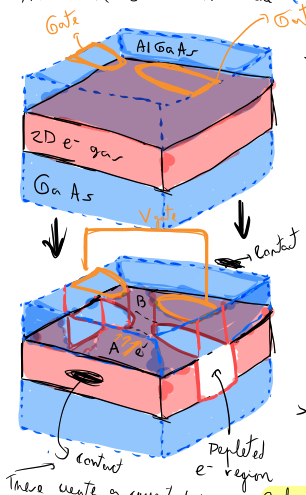
\includegraphics[width=0.3\linewidth]{figures/report_04_2025/qpc_schema.png}
        \caption{Schematic representation of a typical QPC setup \sj{(This is just a placeholder for now)}}
\end{figure*}\label{fig:qpc_schema}

QPC's have garnered significant interest due to their extreme sensitivity to external electric 
fields \cite{fieldMeasurementsCoulombBlockade1993} and the fact that
they exhibit conductance quantization depending on the width of the constriction \cite{wharamTransportQuantisation1988,
vanweesQuantizedConductancePoint1988,
tekmanTheoreticalStudyTransport1991}. The former is of special relevance to this work, as the QPC's are capable of 
sensing individual electrons and performing weak-measurements on systems involving transport. Such a setup has been studied extensively via
a rate equation formalism in \cite{gurvitzMicroscopicDerivationRate1996a,gurvitzNoninvasiveDetector1997a}, with the 
goal of differentiating between classical and quantum transport due to coherence effects, and approach including 
post-selection is shown in \cite{korotkovSelectiveQuantumEvolution2001} in the case of continuous
measurement, weak measurements. These works are discussed in more detail in section \ref{sect:weak_measurements}. 

Furthermore, in the realm of quantum computing, 
QPC's have been proposed as quick and efficient qubit readout devices \cite{engelMeasurementEfficiency2004},
suggesting a reliable method of converting the quantum information stored in qubits into classical information  
(\sj{discussion for experimental realizations}). 

The focus of this study is to build an understanding of the measurement process through a microscopic model of a QPC 
acting as a detector coupled to a double dot system. Section \ref{sect:weak_measurements} introduces the main ideas behind
weak measurements and discusses some of the existing literature surrounding their application to QPC's. Afterwards, 
section \ref{sect:microscopic_model} presents our microscopic model, consisting of a tight binding Hamiltonian for the 
QPC with a local coupling to a double dot. Both detector and system are populated by a single spinless electron at all 
times. 
Here, the main theoretical analysis tools are also introduced. 
Finally, section \ref{sect:numerical_analysis} shows numerical 
results, obtained via exact diagonalization and contrasts them with the analytical predictions.

\section{Weak Measurements}\label{sect:weak_measurements}

The so-called measurement problem in quantum mechanics, is arguably one of the most important open questions
in physics. The associated collapse 
postulate has been the subject of many debates and discussions since the advent of quantum mechanics in the early XX century, 
due to the profound implications it has on the underlying reality \cite{bellsocks1981}. 
The typical statement is as follows: The
wavefunction of a quantum system consists of a 
superposition of states which evolve deterministically 
and unitarily in time according to Schrödinger's 
equation \cite{schrodingerQuantisierung1926,heisenbergUeberQuanten1985}. Yet, at the 
moment of measurement, this superposition collapses to a final state in a fundamentally 
probabilistic process. However, and to complicate
matters further, it is also possible to conduct measurements without bringing about 
a collapse of the wavefunction. Such a measurement is referred to as a \textit{weak/nom-invasive measurement}, in contrast to the usual \textit{projective measurement}.

In the following, we show how weak measurements arise via the ancilla scheme, and discuss the regime
in which they are realized. Afterwards, we present the concept of weak values by adding 
post-selection to non-projective measurements. We finish this 
section with a discussion the application of weak values to systems involving QPC's.

\subsection{The Ancilla Measurement Scheme}

Weak measurements do not require extensions to the axioms of quantum mechanics; in fact, they can be obtained simply by treating the detector device on the same footing as the measured system. Mathematically, this is done by adding terms to the Hamiltonian that represent the detector and its interaction with the system as 
\begin{align}
 \hat{H} = \hat{H}_S + \hat{H}_D + \hat{H}_{I}
\end{align}
where $\hat{H}_S $, $\hat{H}_D $, $ H_{I}$ correspond to system, detector and interaction Hamiltonian respectively. 
Initially, system and detector are prepared completely independent to each other. Then, they are correlated via unitary 
time evolution through their interaction Hamiltonian, in a process called the \textit{pre-measurement}. Finally, the \textit{read-out} is performed by performing a 
projection only the detector. The system will in turn be affected 
by this projection, however under the right conditions, it will still remain in a superposition of states with minimal change.
The specific way of realizing this process is called the ancilla scheme. 

Following \cite{svenssonPedagogicalWeak2013}, the ancilla scheme starts with the initial uncorrelated 
state written as the density Matrix
\begin{align}
    \hat{\rho_0} =  \hat{\rho_S} \otimes  \hat{\rho_D}
\end{align}
where the reduced density matrices of the system $\hat{\rho_S} = \ket{\psi_{\rm S}} \bra{\psi_{\rm S}}$ and detector 
$\hat{\rho_D} = \ket{\phi_{\rm D}} \bra{\phi_{\rm D}}$ are prepared in some arbitrary pure state. In the pre-measurement, they 
become correlated via the usual time evolution operator $\hat{U} = \exp{ -\frac{i}{\hbar} \int dt \, \hat{H}}$. It is
also assumed that the intrinsic Hamiltonians of the system and detector vanish \cite{PreskillQuantum,svenssonPedagogicalWeak2013,tamirWeakMeasurements2013} 
\sj{(I still don't understand why)}, 
such that only the interaction Hamiltonian appears in $\hat{U}$. This Hamiltonian is assumed to be
\begin{align}
    \hat{H}_{I} = \lambda (t) \hat{S} \otimes \hat{M}
\end{align}
where $\lambda$ is the coupling constant, $\hat{S}$ is the observable of the system we want to measure and $\hat{M}$
is some observable of the detector (also called the pointer). In addition, as quantum non-demolition is required \cite{svenssonPedagogicalWeak2013} \sj{(I haven't been able to find anything regarding non-demolition or what it actually means)}, 
the measured observable should also fulfill $[\hat{H}_I, \hat{S}]=0$. Accordingly, the time evolution operator is given by 
\begin{align}
    \hat{U} = \exp{ -\frac{i}{\hbar} \int dt \,  \lambda (t) \hat{S}\otimes \hat{M} },
\end{align}
which can be further simplified by the assumption that the system and detector only interact in a 
finite time window. 

A particular version of pre-measurement was already proposed in 1938 by von Neumann in 
\cite{vonNeumannFoundationsQuantum2018}, where $\hat{M}$ is the detector's momentum $\hat{p}$ and the 
coupling is $\lambda (\tau) = \lambda \, (\theta (T) - \theta(\tau - T))$ where $\theta (T)$ is 
the step function and $T$ is the measurement time window. Due to the choice of $\hat{M}$ and $\lambda(\tau)$
von Neumann's approach correlates the state of the system with the position of the detector and the  effective coupling strength becomes dependent on the measurement time $T$. 

For now, we assume the same coupling as von Neumann, but leave an arbitrary $\hat{M}$ for the detector. By expanding
$\hat{S}$ in its diagonal basis $\ket{s}$ with eigenvalues $s$, the time evolved pre-measurement state is expressed as
\begin{align*}
  \hat{\rho}_1 = \hat{U}\hat{\rho}_0 \hat{U}^\dagger & =  \sum_{i,j} \ket{s_i} e^{-\frac{i}{\hbar} \lambda T s \hat{M} } \bra{s_i}
  \left (  \hat{\rho}_S \otimes \hat{\rho}_D \right ) \ket{s_j} e^{-\frac{i}{\hbar} \lambda 
    T s_j\hat{M} } \bra{s_j},
\end{align*}
in terms of its initial density matrix. 
$\hat{\rho}_0$.
Here, it is useful to define the pointer states of the detector 
$\ket{\mu_s}$ and projection operators $\hat{P}_s$ as
\begin{align}
    & \ket{\mu_{s_i}} := e^{-\frac{i}{\hbar} \lambda T s_i \hat{M} } \ket{\phi_{\rm D}} = \sum_m  e^{-\frac{i}{\hbar} \lambda T s m } 
    \alpha_m \ket{m} \\
    & \hat{P}_{s_i} := \ket{s_i} \bra{s_i}
\end{align}
where we have expanded $\ket{\phi_{\rm D}}$ in the eigenstates $\ket{m}$ of $\hat{M}$. It is important to notice that the pointer states do not have to
be orthogonal and in fact, they often are not. Using these definitions,$\rho_1$ becomes
\begin{align}\label{eq:pre_measurement}
    \hat{\rho}_1 = \sum_{i,j} ( \hat{P}_{s_i} \hat{\rho}_S \hat{P}_{s_j} ) \otimes 
    (\ket{\mu_{s_i}}\bra{\mu_{{s_j}}})
\end{align}
Looking at $\hat{\rho}_1$, it is clear that the system and detector have become entangled through $\hat{U}$, as
it is not possible to express the joint density matrix as a product state. The corresponding mixed state of the system
is given by tracing out the detector states
\begin{align}\label{eq:pre_measurement_system_full}
    \hat{\rho}_{S,1} =  \sum_m \bra{m}\hat{\rho}_{1}\ket{m} = \sum_{i,j} \hat{P}_{s_i} \hat{\rho}_{S} \hat{P}_{s_j}
    \bra{\mu_{s_j}} \ket{\mu_{s_i}},
\end{align}
as a result the system now depends on the overlap of the meter states. 

Up until this point, 
no assumption has been made regarding the strength 
of the coupling between the detector and the system, therefore equation \eqref{eq:pre_measurement_system_full} is valid
for both projective and weak measurements. To obtain the correct expression for the weak 
coupling limit, it is useful to go back to
 $\hat{U}\rho_0 \hat{U}^\dagger$ and expand the exponential $\hat{U} = \exp{- i g \hat{S}\otimes\hat{M} }$, for a small effective
coupling constant $g := \frac{1}{\hbar} \lambda T$ up to second order
\begin{align}\label{eq:rho_expansion}
    \hat{\rho}_1  & = \hat{U}\hat{\rho}_0 \hat{U}^\dagger \nonumber \\
            & = \hat{\rho}_0  +i g [ \hat{\rho}_0,  \hat{S}\otimes\hat{M} ] - 
            \frac{g^2}{2}[ [ \hat{\rho}_0,  \hat{S}\otimes\hat{M} ] , \hat{S}\otimes\hat{M}] + \mathcal{O}(g^3),
\end{align}
and trace out the detector to obtain the system's reduced density matrix 
\begin{align*}
    \hat{\rho}_{S,1}  & = \hat{\rho}_S  -  \frac{g^2}{2}[ [ \hat{\rho}_S,  \hat{S}] , 
    \hat{S}] \langle \hat{M}^2\rangle + \mathcal{O}(g^3),
\end{align*}
where we have used the definition of the expectation value 
$\langle \hat{M}\rangle = \Tr{ \rho_D \hat{M}}$ and assumed that $\langle \hat{M}\rangle = 0$. Calculating the
matrix elements yields
\begin{align*}
    \bra{s_i}\hat{\rho}_{S,1}\ket{s_j} = \bra{s_i}\hat{\rho}_{S}\ket{s_j} - \frac{g^2}{2}\langle 
        \hat{M}^2\rangle\left( 
        \bra{s_i}[\hat{\rho}_{S},\hat{S}] \hat{S}\ket{s_j} - \bra{s_i}\hat{S}[\hat{\rho}_{S},\hat{S}] \ket{s_j}   \right)
\end{align*}
which can be simplified by applying the $\hat{S}\ket{s_j} = s_j\ket{s_j}$ and $\bra{s_i}[\hat{\rho}_{S},\hat{S}] \ket{s_j} = \bra{s_i}\hat{\rho}_{S}\ket{s_j} \left( s_i - s_j \right)$ to obtain 
\begin{align}\label{eq:pre_measurement_system_expansion}
    \bra{s_i}\hat{\rho}_{S,1}\ket{s_j} = \bra{s_i}\hat{\rho}_{S}\ket{s_j} \left(1 - \frac{g^2}{2} 
    \langle \hat{M}^2\rangle (s_i - s_j)^2 \right).
\end{align}
The same procedure can be repeated for equation \eqref{eq:pre_measurement_system_full} resulting in 
\begin{align}\label{eq:pre_measurement_system_full_elements}
    \bra{s_i}\hat{\rho}_{S,1}\ket{s_j} =  \bra{s_i}\hat{\rho}_{S}\ket{s_j} \bra{\mu_{s_i}}\ket{\mu_{s_j}}.
\end{align}
Given that both equation \eqref{eq:pre_measurement_system_expansion} and \eqref{eq:pre_measurement_system_full_elements} have to agree (up to second order in $g$), then the overlaps of the 
pointer states have to fulfill
\begin{align}\label{eq:overlap_condition}
    \bra{\mu_{s_i}}\ket{\mu_{s_j}} \overset{!}{=} 1 - \frac{g^2}{2} \langle \hat{M}^2\rangle (s_i - s_j)^2 + \mathcal{O}(g^3)
\end{align}
if a measurement is to be weak. Since the corrections are second order, the pointer states have almost 
total overlap in weak measurements. 
This requirement can be rephrased as the variance in the detector's 
measured observable being larger than the difference between the eigenenergies of the system \cite{tamirWeakMeasurements2013}. 
Such a situation implies
that there is a large statistical uncertainty in the measurement process, which requires multiple repetitions of an experiment in order to obtain precise values of observables. An example of such an experimental setup is quantum tomography \sj{(cite some examples)}.

Now that the pre-measurement has been performed successfully, one can carry through the read-out by performing 
a projective measurement on the detector to some eigenstate $\ket{m_k}$, according to Lüdder's rule 
\begin{align}\label{eq:post_measurement_state}
    \hat{\rho}_1(\ket{m_k}) = \frac{ (\Id_S \otimes \ket{m_k}\bra{m_k}) \hat{\rho}_1 
    (\Id_s \otimes \ket{m_k}\bra{m_k})}{\text{prob}(m_k|\hat{\rho}_1)},
\end{align} 
which is just the usual expression of a state after a projective measurement \cite{PreskillQuantum}, but 
including an element of conditional probabilities in the denominator which should be read as "the probability
of obtaining $m_k$, given the state $\hat{\rho}_1$". This probability can be easily expressed via the usual 
definition complete trace
\begin{align}
    \text{prob}(m_k|\hat{\rho}_1) & = \Tr{ \Id_S \otimes \ket{m_k}\bra{m_k}\hat{\rho}_1} \\ \nonumber 
            & = \sum_{l,i,j} \bra{m_l}\otimes\bra{s_l} \hat{P}_{s_i} \hat{\rho}_S \hat{P}_{s_{j}} 
            \bra{m_k}\ket{\mu_{s_i}}\bra{\mu_{s_j}} \ket{m_k}\ket{s_l}\otimes\ket{m_l} \nonumber \\ 
            & = \sum_{j} \bra{s_j} \hat{\rho}_{S}\ket{s_j} | \bra{m_k}\ket{\mu_j}|^2,
\end{align}
where the treatment of classical probabilities in the last line, is much like what one would expect in a 
classical Bayesian paradigm \cite{svenssonPedagogicalWeak2013}. From \eqref{eq:post_measurement_state} the post-readout reduced density matrix of the system is obtained by tracing out the detector's degrees of 
freedom
\begin{align}
    \rho_{S,1}(\ket{\mu_k}) = \frac{1}{\text{prob}(m_k|\hat{\rho}_1)} \hat{\Omega}_k \hat{\rho}_0 \hat{\Omega}_k^{\dagger},
\end{align}
where we have defined the \textit{measurement operators} $\hat{\Omega}_k :=\sum_{i} \bra{m_k}\ket{\mu_i} \hat{P}_{s_i}$, in terms of the detector states 
overlaps. These measurement operators are POVM's \cite{PreskillQuantum} (Positive Operator Valued
Measures)
\sj{(Show that they are hermitian, positive and sum to 1)}, which are often used to described
generalized quantum measurements. The advantage of writing 
the system's post-measurement reduced density matrix in terms of the
measurement operators, is that it is now clear what is meant by a weak measurement:
 If the pointer states are completely orthogonal,
the sum in $\hat{\Omega}_k$ will have a single term corresponding to $i=k$
and the system will be projected to a single $\ket{s_k}$ state. However,
if one allows the meter states to overlap to the degree dictated by equation \eqref{eq:overlap_condition}, the system will remain in a superposition of states after performing the readout. 

The ancilla scheme, described above has the 
advantage of explicitly showing how the weak and 
projective measurements correspond to different 
limits of the same fundamental process. Furthermore,
it should be evident that no additional axioms have 
been added to quantum mechanics to allow for such 
a generalized measurement theory. One has merely added 
the detector Hamiltonian to Schrödinger's equation.

Nonetheless, it is important to point out that the 
ancilla scheme does not solve the measurement problem
by any means. It merely shifts the issue from the system to the detector.
In the end during the  read-out process, the collapse postulate is once
again invoked in order to extract some amount of classical information from the quantum system. Once
again, von Neumann already admitted this situation \cite{vonNeumannFoundationsQuantum2018} since
the pointer can be added to the Hamiltoninan and in turn another more macroscopic pointer
is needed to collapse the wave function, then one can add another one and so on. 
This approach is taken to the logical extreme in Wigner's friend 
thought experiment \cite{wignerRemarksMindBodyQuestion1995}, where a second researcher is added as a 
pointer to the main researcher's mind, resulting in 
a contradiction between both their recorded results. This paradox arises from the fact that the barrier where the collapse postulate is invoked (the barrier between the quantum and classical
world that is) may be placed arbitrarily, however it may not be 
disposed of, at least in conventional quantum mechanics. 

For the moment we won't dwell much on this issue and continue working from the paradigm
of the ancilla scheme. In the following, we show how weak values are obtained in weak-measurements
by adding an element of conditional probabilities in what is called the \textit{post-selection} 
process.

\subsection{Weak Values}

As mentioned previously, weak values are found in the context of a weak measurement with post-selection. What is meant by post-selection is but an application of Bayes theorem for 
conditional probabilities to a quantum process. Here, only the experiments where the system ends
up in a chosen final states are recorded, such that the resulting expectation values also become 
conditional. 

(\sj{it would be good to include a diagram here for the post measurement})


The basic setup for post-selection is as follows \cite{svenssonPedagogicalWeak2013}: A system is 
prepared in a given state $\ket{s}$, called the \textit{pre-selected state}, and is entangled to 
a detector, such that the composite density matrix is given by 
\eqref{eq:pre_measurement}. Before the read-out can be realized (system and detector are
still entangled), a projective measurement of some state $\ket{f}$, called the \textit{post-selected state}, is carried out on the system
\begin{align}
    \hat{\rho}_1 (\ket{f}) = \frac{1}{\text{prob}(f|\hat{\rho}_1)} (\hat{P}_f \otimes \Id_D )
    \hat{\rho}_1 (\hat{P}_f \otimes \Id_D )
\end{align}
as dictated by Lüdder's rule \eqref{eq:post_measurement_state}. This step, is interpreted as only recording the 
experimental realizations in which the system ends up in the states $\ket{f}$, hence the name
post-selection. Given that the system and detector where both entangled before this step,
the detector's reduced density matrix is changed as 
 \begin{align}
    \hat{\rho}_{D,1} (\ket{f}) & = \frac{1}{\text{prob}(f|\hat{\rho}_1)}\Tr_S{(\hat{\rho}_1 (\ket{f}) } \nonumber\\
    & =\frac{1}{\text{prob}(f|\hat{\rho}_1)}|\bra{f} \ket{s}|^2\left[\hat{\rho}_D+2 g \Im\left(S_w \hat{M} \hat{\rho}_D\right)- \right. \\
    &\left. - g^2 \Re\left(\frac{\bra{f} \hat{S}^2\ket{s}}{\bra{f} \ket{s}} \hat{M}^2 \hat{\rho}_D-\left|S_w\right|^2 \hat{M} \hat{\rho}_D \hat{M}\right)\right] + \mathcal{O}(g^3) \nonumber
\end{align}
where we used the expansion \eqref{eq:rho_expansion}, assumed $\bra{f}\ket{s}\neq 0$ and defined the weak value 
\begin{align}
    S_w := \frac{ \bra{f} \hat{S}\ket{s} }{\bra{f}\ket{s}}.
\end{align}
The probability of obtaining $f$ given $\hat{\rho}_D$ is given by 
\begin{align}
    \text{prob}(f|\hat{\rho}_1) = \bra{f}\ket{s}^2 \left[  1- g^2 \langle \hat{M}^2\rangle
        \Re{ \frac{\bra{s} \hat{S}^2\ket{s}}{\bra{f}\ket{s}} - |S_w|^2} \right].
\end{align}
Notice that the definition of $S_w$ implies that weak values may be complex numbers. 

From this conditional reduced density matrix we may now calculate the conditional
expectation value of some detector observable $\hat{L}$ as 
\begin{align}\label{eq:conditional_expectation}
    \langle \hat{L}\rangle_{f} = \langle \hat{L} \rangle_0 + g \Im{S_{w}\langle \hat{L}\hat{M}\hat{\rho}_{D} \rangle \frac{1}{\text{prob}(f|\hat{\rho}_1)}},
\end{align}
where $\langle \hat{L} \rangle_0$ is used to denoted the expectation value of $\hat{L}$ without post-selection. This result shows some remarkable properties of weak values. First, notice that 
equation \eqref{eq:conditional_expectation} implies that weak values can be directly measured in 
an experiment, despite the fact that they may be complex numbers. This property has been exploited
to directly measure the wavefunction \cite{lundeenDirectMeasurementQuantum2011} without the use 
of quantum tomography. Second, a suitable choice of $\ket{f}$, 
for example such that $\bra{f}\ket{s}$ is very small, may cause the conditional expectation value 
of an observable to become extremely large, a phenomenon known as amplification. In fact, weak values were first defined in Aharonov, Albert and Vaidman's seminal paper 
\cite{aharonovHowResultMeasurement1988}, where the authors showed how a judicious choice of $\ket{f}$
can result in spin measurement way beyond the forbidden region. It must be pointed out however that
amplification involves pots-selecting very rare states \cite{svenssonPedagogicalWeak2013}.

Such seemingly nonsensical results (among other) have sparked a debate on the validity of weak 
values and whether they correspond to actual physical properties of a system. Regardless of the 
ontological status of weak values, it is clear that they correspond to
statistical quantities intrinsically linked to both the pre- and post-selected state 
\cite{alonsoQuantumAveragesWeak2005} which accurately
predict observable physical phenomena  \sj{(I don't want to 
fully dive into this rabbit hole but there needs to be more here)}.

Among other concrete applications of weak measurements and values, most relevant to this work 
are their application to QPC systems. 

\subsection{Non-invasive measurements on QPC's}

Gurvits and Korotkov 

Oded's paper linked to chesire cat

\section{Microscopic Model of a Double Dot measurement}\label{sect:microscopic_model}

Our experimental set-up of interest consists in a QPC coupled to an isolated double dot (DD), much like 
those described in the previous section. However, we focus on a microscopic description of this
detector-system by modelling the QPC as an  $N$-site tight binding chain with a local interaction
to a double dot Hamiltonian
\begin{align}\label{eq:qpc_dd_H}
    H = -\sum_{j}J_{j}(a_{j}^{\dagger} a_{j} + a_{j+1}^{\dagger}a_{j} ) - 
    t(d_{2}^{\dagger}d_{1}+d_{1}^{\dagger}d_{2}) +  \Omega \, d_{1}^{\dagger}d_{1}( a_{b}^{\dagger}a_{b+1} 
    + a^{\dagger}_{b+1}a_{b} ),
\end{align}
where $J_j$ is the QPC hopping, $t$ is the double dot hopping and $\Omega$ is the coupling between 
both, which acts on the site $b$ referred to as the bond. The ladder operators for the QPC 
and DD $a_j$ and $d_k$ are fermionic. This simple model allows for an exact solution in the decoupled case 
as well as an approximate analysis with scattering theory and the ancilla scheme 
as described in section \ref{sect:weak_measurements}.

First, we derive the exact solution for the decoupled case in section \ref{sect:decoupled_system}.
Then, we follow up in \ref{sect:scattering} with an approximate analysis for
slow double dot dynamics, by reducing the problem to one of 
scattering from a delta potential, providing an estimation of the relevant timescales. 
Finally, in section \ref{sect:bloch_backaction} we study the back-action of the 
QPC on the double dot using von Neumann measurements in the ancilla scheme. 

\subsection{Decoupled system}\label{sect:decoupled_system}

For the case were QPC and DD are decoupled ($\Omega = 0$) it is possible to diagonalize the 
Hamiltonian of each part analytically. 

For the QPC, we assume uniform hopping $J_j = J$ and open boundary conditions. Accordingly, 
The matrix form of the Hamiltonian in the lattice site basis $\ket{j}$ is 
\begin{align}
    H_{\text{QPC}} = 
    \begin{pmatrix}
        0 & -J  & 0 & 0 \hdots & 0 \\
        -J & 0  & -J & 0 \hdots & 0 \\
        0 & -J  & 0 & 0 \hdots  & 0 \\
        \vdots &  &  & \ddots & \vdots \\
        0 &  & \hdots & 0& -J \\
        0 &  & \hdots &  -J & 0 
    \end{pmatrix}
\end{align}
which can be diagonalized  by solving the algebraic equations 
\begin{align*}
    v_{j+1} + E v_j + v_{j+1} = 0 , \quad j = 1,2, \hdots , N ; \; v_0 =v_{N+1} = 0
\end{align*}
for the eigenvector components $\vec{v} = (v_1, v_2, \hdots, v_N)$ and the $E$ eigenenergies. 
The eigenvectors and energies are given by
\begin{align}\label{eq:tight_binding_sol}
   & \vec{v}(k) = \begin{pmatrix}
        v_1(k) \\
        v_2(k) \\
        \vdots \\
        v_N(k)
    \end{pmatrix} , \; v_j(k) = \bra{v_k}\ket{j} = \sin(k j), \; k=\frac{\pi}{N+1} n , 
    \; n = 1, \hdots , N \\
    & E(k) = -2J\cos(k)
\end{align}
in terms of the wavevector $k$ as. We can now use these eigenvectors to find the time evolution of the 
system, starting from the initial vector in position basis
\begin{align}\label{eq:qpc_gauss_lattice}
        \ket{\psi(0)} = \sum_{j=1}^N \alpha_j \ket{j}
\end{align}
where $|\alpha_j|^2$ gives the probability of being at site $j$ at time $\tau=0$ for the QPC particle. 
Plugging in the abstract eigenvectors with $\Id = \sum_k \ket{v_k}\bra{v_k}$ and using the definition 
of $v_j(k)$ yields
\begin{align*}
    \ket{\psi(0)} = \sum_{j,k}^N \alpha_j v_j(k)\ket{v_k},
\end{align*}
which may now by multiplied by the time evolution operator in its diagonal basis to obtain the expression
\begin{align}
    \ket{\psi(\tau)} = e^{-i/\hbar \hat{H}} \ket{\psi(0)} = 
            \sum_{k=1}^N \vec{\alpha}\cdot \vec{v}(k) e^{-i/\hbar\tau E(k)} \ket{v_k}
\end{align}
for the wavefunction at a time $\tau$.

In our case, we want to represent the QPC particle as a travelling wave packet. Therefore, the $\alpha_j$
coefficients are taken from the Gaussian distribution
\begin{align}\label{eq:gaussian_distribution}
    \alpha_{j}=\left(\frac{1}{\pi \Delta^2}\right)^{1/4}e^{-\frac{1}{2\Delta^2}(aj-x_{0})^2 + i k_0 (x-x_0)}
\end{align}
where $a$ is the lattice spacing, $k_0 = p/\hbar$ is the average momentum and $\Delta$, 
controls the degree of localization 
around $x_0$, which
may be interpreted as the initial position.

For the case of the decoupled double dot, the Hamiltonian reduces to that of a simple two level system 
\begin{align}
    H_{\text{DD}} = \begin{pmatrix}
        \epsilon_0 + \delta & -t \\
        -t & \epsilon_0 - \delta 
    \end{pmatrix}
\end{align}
where we have added the diagonal energies and detuning to justify the following useful parametrization . 
The characteristic equation yields the eigenvalues $\lambda_{\pm} = \epsilon_0 \pm \sqrt{\delta^2 + t^2}$
and their corresponding normalized eigenvectors are commonly expressed in terms of trigonometric 
functions as
\begin{align}
    & \ket{+} = \begin{pmatrix}
      \cos(\beta/2) \\
        e^{i\eta} \sin(\beta/2) 
    \end{pmatrix} , \quad \ket{-} = \begin{pmatrix}
        \sin(\beta/2) \\
          -e^{i\eta} \cos(\beta/2)
      \end{pmatrix} 
\end{align}
where $\sin(\beta) = t /\sqrt{\delta^2+t^2 }$ and $\cos(\beta) = \delta /\sqrt{\delta^2+t^2}$ and 
$\eta$ is an arbitrary phase that acts as a free parameter. Using these eigenvectors, the position 
basis is expressed as
\begin{align}
    & \ket{0} = \cos (\beta/2) \ket{+} + \sin(\beta/2) \ket{-} \\
    & \ket{1} = e^{-i \eta} \sin (\beta/2) \ket{+} - e^{-i \eta}\cos(\beta/2) \ket{-}. 
\end{align}

As mentioned before, since the actual Hamiltonian is \eqref{eq:qpc_dd_H}, the energies and detuning are 
chosen as $\epsilon_0 = \delta = 0$ for the rest of this work. It is however useful to keep the 
trigonometric functions (specially when dealing with the Bloch representation)
and only use the explicit form until the end of a calculation. Hence, we shall keep them.

As is usual with such two-level systems, they will exhibit Rabi oscillations between the two $\ket{0}$ and
$\ket{1}$ states. To see this, assume that the double dot starts in the $\ket{0}$ state. At 
a later time, it will be at 
\begin{align*}
    \ket{\psi (\tau)} = e^{-i/\hbar \hat{H}_{DD}}\ket{0} & = 
        e^{-i/\hbar \tau\lambda_{+}}\cos (\beta/2) \ket{+} + 
        e^{-i/\hbar \tau \lambda_{-}}\sin(\beta/2) \ket{-} 
\end{align*}
and the probability of being in the state $\ket{1}$ at time $\tau$ will be
\begin{align}
    P(\ket{1})_\tau = |\bra{1}\ket{\psi(\tau)}|^2 = \sin^2(\omega\tau),
\end{align}
where we defined $\omega := \frac{1}{\hbar}t$ as the Rabi frequency.

For a general initial state and $\epsilon_0 = \delta = 0$, the wavefunction of the DD at a 
later time will be given by 
\begin{align}\label{eq:DD_wave_general}
    \ket{\psi (\tau)} = \frac{1}{\sqrt{2}}\left( A_0  +B_0 e^{-i\eta} 
    \right) e^{-i\tau \lambda_+} \ket{+} + 
    \frac{1}{\sqrt{2}}\left( A_0  -B_0 e^{-i\eta} 
    \right)  e^{-i\tau \lambda_-} \ket{-}.
\end{align}

The exact equations we just derived for the decoupled QPC-DD will be useful later, when we develop
approximate analysis in the coupled case at different limits and for building a numerical solution.
In the next section we now develop an approximate description of the QPCS-DD system involving a travelling
Gaussian wavepacket that scatters off a constant delta potential.   

\subsection{Scattering analysis and timescale estimation}\label{sect:scattering}

Given that the Hamiltonian \eqref{eq:qpc_dd_H} is too difficult to solve for an $N$-sites, one has to resort to approximations to continue the analysis. A first approach is to reduce the system to a one dimensional scattering problem from a delta potential.
As will be shown below, this approach has the advantage of illustrating the conditions that the 
Gaussian QPC particle has to fulfill in order to have a true measurement process. In addition, 
we will also able to quantify the relevant time-scales of the system. 
We will focus more on the general procedure rather than the detailed calculation, 
in order to make the assumptions more explicit.

For starters, the QPC tight-binding chain has to be long enough, such that its initial 
state is that of a free particle with energy $E_0 = \hbar^2 k_0^2/2m$ and is completely 
independent of the
double dot. Additionally, it is assumed that the Rabi oscillations in the double dot are 
slow enough, so the coupling is approximately constant \sj{(what exactly is meant by slow enough will be made clear later)}. In this
situation, the problem can be expressed in the continuum as the usual time independent Schrödinger
equation 
\begin{align*}
    -\frac{\hbar}{2m} \frac{d^2 \psi (x)}{dx^2} - V_0 \delta(x) = E \psi (x),
\end{align*}
where the interaction with the double dot is reduced to a delta potential since it only acts directly at
the bond, and $V_0$ is the effective coupling. At $\tau = 0$ the QPC particle is given by the Gaussian 
\begin{align}\label{eq:gaussian_packet}
    \Psi(x,0) = \left(\frac{1}{\pi \Delta^2}\right)^{1/4} \exp{ -\frac{(x+x_0)^2}{2\Delta^2} +
     i k_0 (x+x_0)},
\end{align}
where we assumed that the particle is initially located at $-x_0$. This wave packet is formed 
by a proper superposition of plane waves at different momenta. 
In addition, to have a scattering event 
the above wave packet needs to have well-defined trajectories i.e $\Delta$ is large enough that 
the wave function is sharply
peaked around $k_0$ in momentum space, according to $\Delta_k = \hbar/\sqrt{2}\Delta$. 
We now proceed, following Shankar \cite{shankarQuantumMechanics1994}, to calculate the transmision
rate.

Since each $k$ interacts differently with the potential, one may solve Schrödinger's equation 
for each individual plane wave (which are the eigenfunctions), 
By noticing that to the left and right of the potential, the solution is that of a free particle. 
To the left of the barrier
there is an incident and a reflected wave $\Psi_{L}(x,k) = A e^{ik x} + B ^{-ikx}$, while to the right 
it is assumed that there is only a transmitted one $\Psi_{R}(x,k) = C e^{ik x}$.

The explicit forms of $A$, $B$ and $C$ are found by imposing continuity conditions at $x=0$ on $\psi$ 
and its derivates. These eigenfunctions also give the transition rate 
\begin{align}
    T(k) = \int |\psi_R (k,x)|^2 = \frac{1}{1+\frac{m^2 V_0}{\hbar^4 k^2}} 
\end{align}
for a plane wave with momentum $k$.

The plane wave eigenstate $\psi_E(x,k) = \Psi_{L}(x,k) + \Psi_{R}(x,k)$, yields the 
times evolution of the Gaussian wavepacket $\psi(x,0)$ by its projection $a(k) = \bra{\psi_e}\ket{\psi}$
to each individual $k$ as 
\begin{align*}
    \psi (x,\tau) = \int_{-\infty}^{\infty} dk \; a(k) e^{-i \tau/\hbar E(k)} \psi_e(x,k).
\end{align*}
Given that, in scattering problems one is mostly interested in the transmission rate,
one takes the $t\rightarrow\infty$ limit in addition to assuming large $\Delta$. 
As is shown by Shankar, only plane waves survive these two limits. Therefore, the total transition rate
is just the weighted sum of the rates from each individual $\psi_e(k)$
\begin{align}\label{eq:transmision_coef}
    T = \int dk \; T(k) |\tilde{\psi}(k,0)|^2
\end{align}
where $\tilde{\psi}(k,0)$ is the Fourier transform of the initial Gaussian wave packet
\begin{align}
    \Psi(x,0) = \left(\frac{\Delta^2}{\pi}\right)^{1/4} \exp{ -\frac{\Delta^2(k-k_0)^2}{2} + i k x_0}.
\end{align}
Notice how, in calculating the transition rate one assumes a stationary process. How may one reconcile this situation with a quantum measurement, where time plays 
an important role? This is an issue of determining what it means to take time to "infinity" 
in a finite QPC. A suitable choice is suggested by the assumption that the transmitted
wave has no reflections from the far wall of the chain. Hence, our operational definition of "infinite
time" is the time it takes for the QPC particle to hit the end of the tight-binding chain. Since 
the travelling wave behaves as a free particle, up until the point it hits the bond, we may
 approximate the hitting time by using Ehrenfest's theorem 
\begin{align}
    \tau_f = \frac{m \langle L \rangle }{ \langle p \rangle} = \frac{L}{v_g}
\end{align}
where $L$ is the length of the chain and $v_g$ is the group velocity. 

This $\tau_f$ and the assumptions we made in the above calculations are specially relevant for numerical
simulations, which warrants listing them again: 
\begin{enumerate}
    \item The QPC tight binding
    chain is long enough such that the initial state can be considered completely 
    independent of the double dot.
    \item The wave packet has well-defined trajectories, meaning $\Delta$ has to be large such that 
        the momentum 
        distribution is sharply peaked. However, in a finite system it cannot be too large, otherwise the
        QPC wavefunction overlaps with the bond and assumption  1 is no longer valid.
    \item There can be no reflections coming from the end of the chain, so the measurement process has to
        end before $\tau_f$ as defined above.
    \item The double dot dynamics are slow enough to be considered constant 
\end{enumerate}
Assumption number 4 can be relaxed (and in fact it will be) when considering situations going beyond 
the time-independent scattering regime. On the other hand, assumptions 1 and 3 are specially 
important for a measuring process as presented in section \ref{sect:weak_measurements}, 
since one always assumes the systems start unentangled and reflected waves will 
cause secondary entanglement events during the pre-measurement. Regarding $V_0$, it will be a 
function of both $\Omega$ and the time-window in which the pre-measurement takes place \sj{(i
still have not figured this one out yet)}.

The previous scattering calculation has focused solely on the quantum point contact. While it is now 
clear that a proper spread $\Delta$ is needed to have a well-defined trajectory (and therefore a 
measurement time-window) and the measurement has to end before the QPC particle hits the end of the 
chain, this approach cannot say anything about entanglement production because it completely 
neglects the double dot's dynamics. In the next section, we will turn to the double dot and 
quantify the backaction of such a Gaussian wave packet by using von Neuman measurements in the 
ancilla scheme.


\subsection{Bloch Sphere representation and backaction}\label{sect:bloch_backaction}

In this section we apply the concept of 
von Neuman pre-meassurement, developed in section \ref{sect:weak_measurements}, to the QPC-Double dot case. We will use the Bloch-Sphere representation to quantify the 
backaction induced by the QPC and find an 
expression for the reduced density matrix 
of the double dot which will be used to 
calculate entanglement in numerical simulations.

Initially, both DD and QPC are in the product state 
\begin{align*}
    \hat{\rho} = \ket{\psi_{DD} }\otimes \ket{\psi_{\rm QPC}(x_0)}\bra{\psi_{\rm DD} }\otimes \bra{\psi_{\rm QPC}(x_0)}
\end{align*}
where $\psi_{DD} = A_0 \ket{0} + B_0 \ket{1}$ and $\ket{\psi_{\rm QPC}}$ is the Gaussian 
\eqref{eq:qpc_gauss_lattice} in the position basis. Since the double dot is a two level system, it can be 
represented in the Bloch Sphere as 
\begin{align}
    \hat{\rho}_{DD} = \frac{1}{2}\left( \Id_{\rm DD} + \vec{q}\cdot\vec{\sigma} \right)
\end{align} 
where $\vec{q} = (\sin(\theta)\cos(\phi), \; \sin(\theta)\sin(\phi), \; \cos(\theta))^T$ is the
Bloch vector and $\vec{\sigma} = (\hat{\sigma}_x, \hat{\sigma}_y, \hat{\sigma}_x )$ is 
a vector of Pauli matrices. Its free evolution is expressed as the change of the Bloch
angle $\theta(t) = -\theta_0+2\omega\tau$ depending on the Rabi frequency $\omega=-t/\hbar$ and 
$\phi$ is an arbitrary constant. To make the notation clearer, we suppress the time dependency in $\theta$ until
the end of the following calculation.

In order to entangle the QPC and DD, the unitary time evolution is expressed, following the 
ancilla scheme and von Neumann as
\begin{align}
    \hat{U}(T) \approx & e^{i\Omega T \hat{\sigma}_z \otimes \hat{p}} \\
            & = \ket{0}\bra{0} e^{-\Omega T \hat{P}} + \ket{1}\bra{1} e^{\Omega T \hat{´}}
\end{align}
where the system's observable is its position (measured by $\hat{\sigma}_z$) and it is coupled to the momentum 
$\hat{p}$ of the QPC for the duration $T$ of the measurement. 
Here we have set $\hbar=1$ and will continue using this notation. Notice that, this form of $\hat{U}$ assumes that
the pre-measurement happens quickly enough such that, the intrinsic Hamiltonians may be left out \sj{(This is 
the assumption that bothers me the most)}.
Applying this unitary operator to the initial state yields
\begin{eqnarray}
    \ket{\Psi_1} = \cos(\theta/2) \ket{0}\otimes \ket{\psi_{\rm QPC}(x_0-\Omega T)} + 
                    \sin(\theta/2) e^{i\phi}\ket{0}\otimes \ket{\psi_{\rm QPC}(x_0+\Omega T)}, 
\end{eqnarray}
by using the fact that $\hat{p}$ is a generator of translations in position space \cite{vonNeumannFoundationsQuantum2018} \sj{(Jeff raised a good question here and is if
in the numerics we are really coupling to the position?)}. 
As is expected, the pre-measurement state is entangled. The reduced
density matrix of the dot can then be found by tracing out the detector states with its position basis
\begin{align*}
    \hat{\rho}_{1,DD} = \sum_{m} \left(\Id_{\rm DD}\otimes \bra{x_m}\right)  \ket{\Psi_1} \bra{\Psi_1}
    \left(\Id_{\rm DD}\otimes \ket{x_m}\right)
\end{align*}
where each $\ket{x_j}$ corresponds to a lattice site $j$. Notice that the projection of the QPC state onto 
the position basis $\bra{x_m}\ket{\psi_{\rm QPC}(x_0\pm\Omega T)} = \psi(x_j, x_0\pm\Omega T)$ is just the same 
Gaussian as \eqref{eq:gaussian_packet} but centered around $x_o \pm \Omega T$. The expression then becomes
\begin{align*}
        \hat{\rho}_{1,\rm DD}^{\prime}=  \sum_m & \left\{\cos^2 \frac{\theta}{2}\left| \psi(x_j, x_0-\Omega T)\right|^2\ket{0} 
        \bra{0} \right. \\
        &\left.+\sin\frac{\theta}{2} \cos\frac{\theta}{2} e^{-i \phi} \psi(x_j, x_0-\Omega T)
        \psi^*(x_j, x_0 + \Omega T) \ket{0}\bra{1}  \right.\\
        &\left.+\sin\frac{\theta}{2} \cos\frac{\theta}{2} e^{i \phi} \psi(x_j, x_0+\Omega T)
        \psi^*(x_j, x_0 - \Omega T) \ket{0}\bra{1}  \right.\\
        & \left. +\sin^2 \frac{\theta}{2}\left| \psi(x_j, x_0+\Omega T) \right|^2 \right\}.
\end{align*}
The $\psi$ in the diagonal elements sum to one. 
Meanwhile, the cross terms can be explicitly calculated by turning the 
sum over $m$ \sj{(lay be less confusing to just start with the integral at the trace)} into an integral over $x$ as
\begin{align*}
    \sum_m \psi(x_j, x_0-\Omega T)
    \psi^*(x_j, x_0 + \Omega T) \rightarrow & \frac{1}{2\pi\Delta^2} e^{-2(\Omega T/\Delta)^2+2ik_0T} \int dx 
    \; e^{-1/\Delta^2 (x-x_0)^2} = \\
    & = \frac{1}{\sqrt{2}} e^{-2(\Omega T /\Delta)^2} e^{2ik_0T\Omega} = R e^{i\gamma} 
\end{align*}
where we defined the amplitude as $R:= e^{-2(\Omega T /\Delta)^2} $ and 
the phase as $\gamma := 2 k_0 T \Omega$. The other cross term is
just the complex conjugate
\begin{align*}
    \sum_m \psi(x_j, x_0+\Omega T) = R e^{-i\gamma}.
\end{align*}
Putting it all together in matrix form
\begin{align*}
    \hat{\rho}_{1,\rm DD} = 
    \begin{pmatrix}
        \cos^2(\theta/2)& \cos(\theta/2) \sin(\theta/2) R e^{-i(\phi-\gamma)} \\
        \cos(\theta/2) \sin(\theta/2) R e^{i(\phi-\gamma)} & \cos^2(\theta/2), 
    \end{pmatrix}
\end{align*}
can be rewritten in the Bloch form by using trigonometric identities and the definition of the Pauli
matrices to obtain
\begin{align}
    \hat{\rho}_{1,\rm DD} = \frac{1}{2} \big( \Id + \vec{q}_1 \cdot \vec{\sigma} \big), \qquad 
    \vec{q}_1 = \begin{pmatrix} R \sin(\theta)\cos(\phi -\gamma) & R \sin(\theta)\sin(\phi -\gamma)  
                            \cos(\theta) \end{pmatrix}^T 
\end{align}
described by the new Boch vector $\vec{q}_1$. It is here that the effect of the 
pre-measurement is made evident. 
First, due to $R$ the magnitude of $\vec{q}_1$ is now less than one, 
as expected of a mixed system due to a loss of purity. Additionally, the double dot has acquired an extra phase 
$\gamma$, meaning that the orbit traced due to Rabi oscillations will be rotated around the $z$-axis 
compared to the initial state. Furthermore, this phase not only depends on the 
measurement time $T$, and coupling strength $\Omega$, but also on the central momentum of the wave packet $k_0$. 
The meaning of this will be made clearer in the next section with the discussion of the numerical results.
Interestingly, there has been no effect on the
Rabi frequency in $\theta (t)$. This is due to our initial assumption of the pre-measurement occurring in a small time window. 
In truth, there is also a change in the frequency, as the numerics will show \sj{(How
can we show this more formally)}.

We have successfully used the pre-measurement of the ancilla scheme to show that the
entanglement backaction of the QPC on the dot produces an extra phase $\gamma$, which is dependent 
on the momentum of the traveling wave. 
Next, we will compare these results with those obtained numerically by exact 
diagonalization. 


\section{Numerical Analysis}\label{sect:numerical_analysis}

Having presented the mathematical formalism behind the microscopic model of the QPC-Double Dot system
and their pre-measurement entanglement, we proceed to compare it with numerical data. All the following results were obtained by applying the exact diagonalization procedures from Qutip 
on the Hamiltonian \eqref{eq:qpc_dd_H} with $L$ lattice sites. 
This allows us to find the time evolution
while keeping our treatment microscopic (i.e. Hamiltonian). For simplicity, we set $\hbar = m =1$.

The QPC particle is always initialized in the far left lattice site $j=0$ as a Gaussian wavepacket
in the position basis as dictated by equation \eqref{eq:qpc_gauss_lattice}, with the $\alpha_j$
coefficients taken from the normal distribution \eqref{eq:gaussian_distribution}. Here,
only the basis states with a single particle are included in the expansion. As discussed in section
\ref{sect:scattering}, special care has to be taken when choosing the spread of the wave packet. 
Preliminary testing has shown that a spread of $\Delta =2 J$ produces a sufficiently localized 
momentum distribution without causing the spatial distribution to overlap with the bond, as the 
wave packet is roughly localized to around 3 lattice sites. This will allow us to have both well-defined trajectories and a time window when the detector interacts with the 
system. In this case, 
the pre-measurement occurs when the QPC particle hits the bond, which is located around the
middle of the chain to avoid reflections. 
In addition, the central momentum of the particle $k_0$ will define the
group velocity, according to the tight-binding energy \eqref{eq:tight_binding_sol} and 
dispersion relation
\begin{equation}
    v_g = \frac{\partial E(k)}{\partial}\Big|_{k_0} = 2 J \sin(k_0)
\end{equation}
where $k_0\in[0,\pi/2]$ due to the periodicity of the sine function.

The double dot is initialized
as $\ket{\psi_{\rm DD}} = A_0 \ket{0} + B_0 \ket{1}$,
where the initial conditions are fixed by 
\begin{align}
    A_0 = \cos\left( t L_B \left(\frac{1}{v_g} - \frac{1}{2J}\right) \right) \\
    B_= = \sin\left( t L_B \left(\frac{1}{v_g} - \frac{1}{2J}\right) \right),
\end{align}
where $L_B$ is the position of the bond. These expressions ensure that regardless of $v_g$, the 
state of the double dot will always be the same when the wave packet hits the bond. This allows 
us to isolate the effect of the different variables from the dot occupation at the start
of the pre-measurement.

The simulation time is set to $\tau_{max}=L/v_g$. By Ehrenfest's theorem, this corresponds 
to the time a free particle will reach the end of the QPC chain, which allows us to reduce finite
size effects due to reflections.

Having set most of the algorithm's parameters, we focus on $\Omega$, $k_0$ and $t$ and their effect
on entropy production and the backaction. All the following results have been obtained with the parameters $L=21$, $\Delta=2$ unless 
explicitly stated otherwise.

An example on the dynamics of the QPC-DD system can be seen in figure \ref{fig:trajectory_example}(a),
where the local densities $\hat{n} = \hat{a}_j^\dagger\hat{a}_j$ are plotted on a heat map,
giving a rough estimate of the trajectories. Here, it is shown how the QPC particle evolves
rather clasically until it hits the bond, where part of it is reflected (notice the faint 
side bands) and another is transmitted until it reaches the end of the chain. Despite truncating
at $\tau_{\rm max}$, reflections from the far wall are still clearly present. 

A closer look is 
presented in figure \ref{fig:trajectory_example}(b). Here, the Rabi oscillations are shown on top
of the sum of the QPC local densities to the left and right of the bond, as well as the bond and 
last site occupations. The sum of the densities to the right is of special interest, because it 
roughly coincides with the transmission rate in the scattering regime. The occupations directly 
at the bond are also quite useful, since they can be used to estimate the pre-measurement time window
as its \textit{Full Width at Half Maximum} (FWHM) $T = \text{FWHM}(\hat{n}_{\rm bond})$. This
graph also shows reflection effects as fluctuations in the bond density, which is expected to 
have a Gaussian-like shape.

\begin{figure}[h]
    \centering
    \begin{subfigure}[b]{0.55\textwidth}
        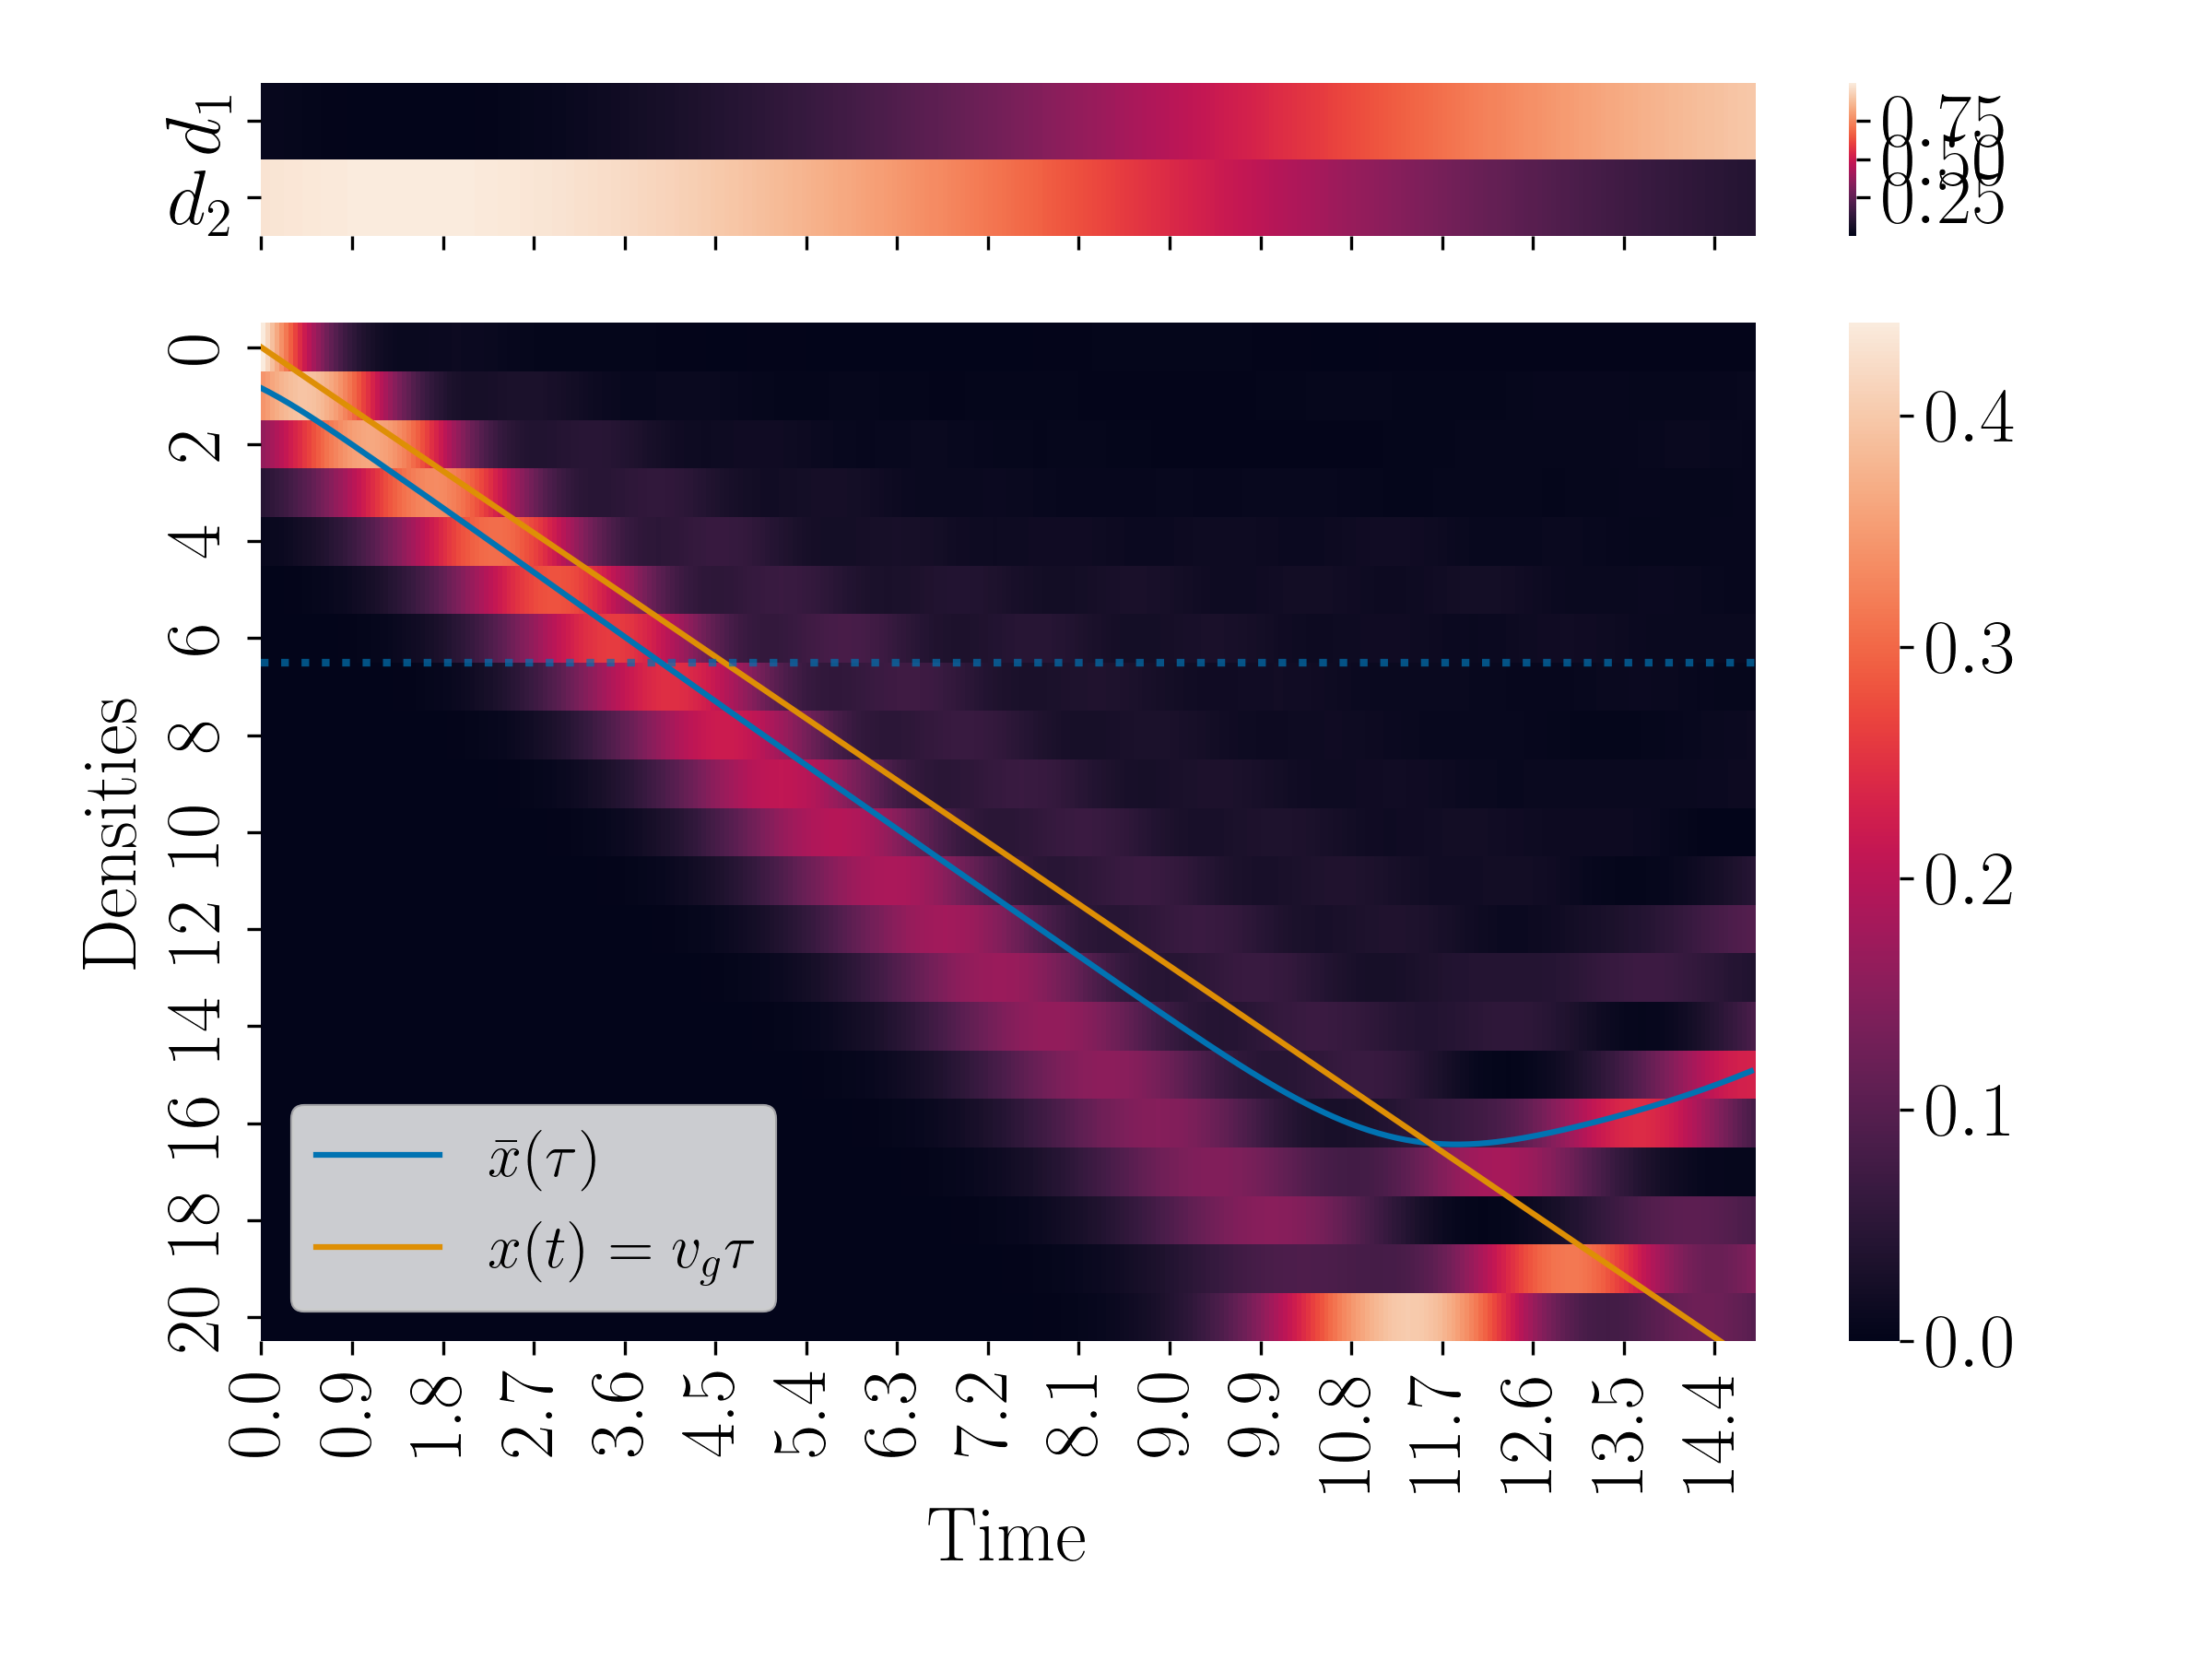
\includegraphics[width=\textwidth]{figures/report_04_2025/traject_ex.png}
        \caption{}
    \end{subfigure}
    \hspace{0.001\textwidth}
    \begin{subfigure}[b]{0.4\textwidth}
        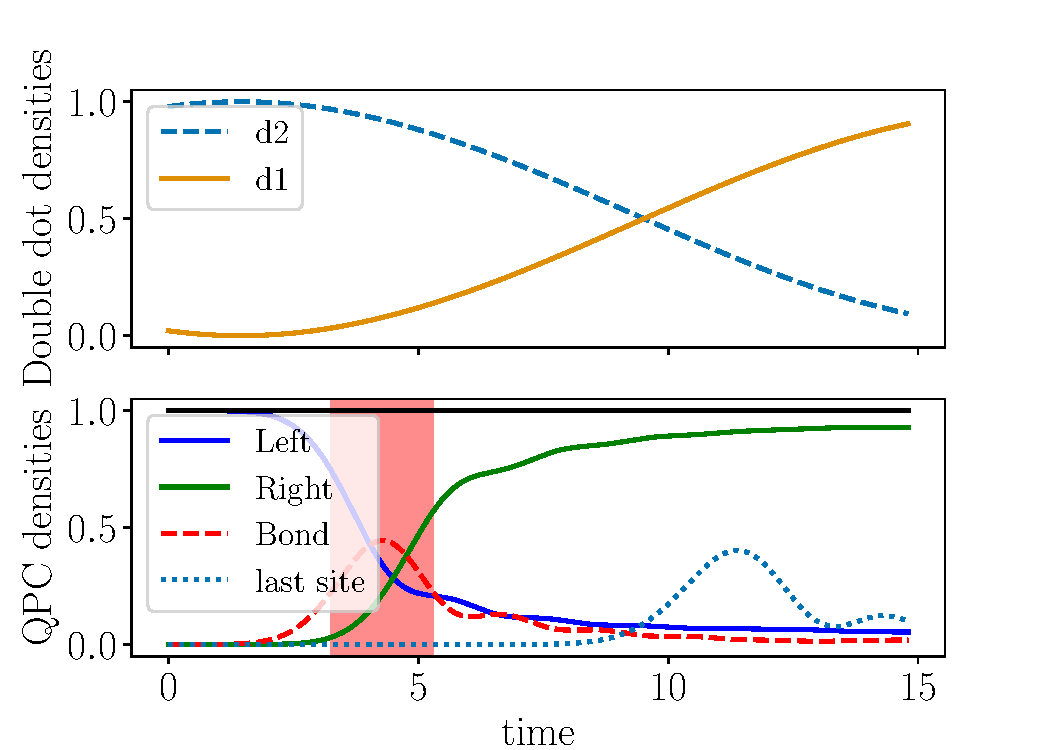
\includegraphics[width=\textwidth]{figures/report_04_2025/densities_ex.pdf}
        \caption{}
    \end{subfigure}
    \caption{Example for a detector-system with $\Omega=0.3$, $t=0.1$ and $k_0=0.79$ . 
    (a) Trajectories in
    time (x-axis) and lattice site (y-axis) for the dot on top and QPC at the bottom. 
    The color of the heat map corresponds to the
    occupation at a given site, the dotted line shows the placement of the bond and the
    solid blue and orange lines show the average position from the numerics and the free particle
    respectively. (b) Occupations as a function of time in the double dot (top) and QPC (bottom).
    For the QPC the different lines correspond to the densities at the bond, at the last site and
    the sum of all sites to the left and right of the bond. The red strip shows the time that 
    the QPC particle spends at the bond estimated via the FWHM of the bond density.}
    \label{fig:trajectory_example}
\end{figure}

Furthermore, for this same example, figure \eqref{fig:bloch_representation} shows the reduced 
density matrix of the double dot in the Bloch sphere. These graphs indicate that, as predicted,
the coupling of the double dot to the QPC induces an extra phase, represented as a rotation around the 
$z$-axis. In addition, figure \ref{fig:bloch_representation}(b) shows that there is also slight modification of the Rabi frequency in $\theta (t)$. It is also clear that there is a 
time window in which 
the interaction between system and detector takes place, as the phase $\phi$ changes rapidly but 
remains almost constant afterwards. 

\begin{figure}[h]
    \centering
    \begin{subfigure}[b]{0.4\textwidth}
        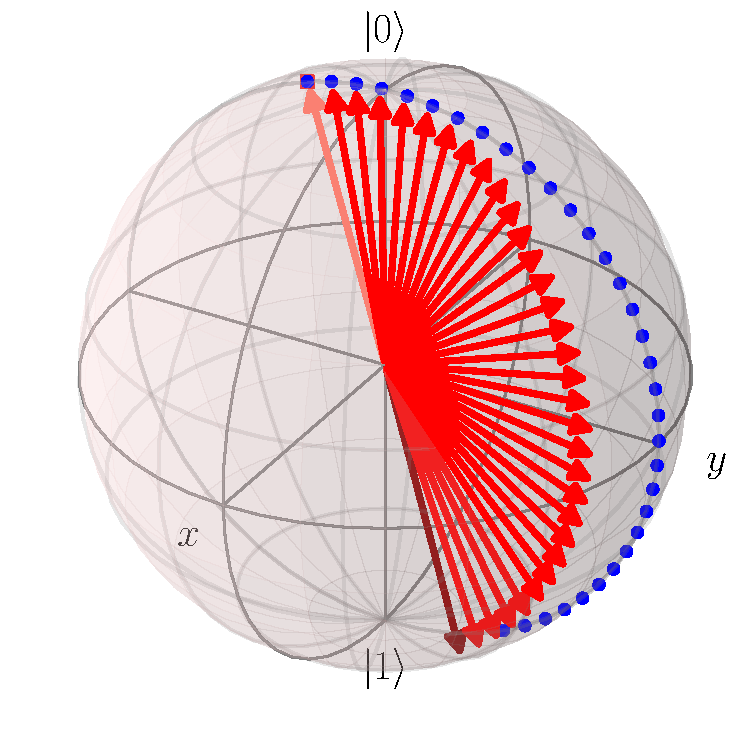
\includegraphics[width=\textwidth]{figures/report_04_2025/bloch_sphere.pdf}
        \caption{}
    \end{subfigure}
    \hspace{0.001\textwidth}
    \begin{subfigure}[b]{0.5\textwidth}
        \includegraphics[width=\textwidth]{figures/report_04_2025/bloch_angles.pdf}
        \caption{}
    \end{subfigure}
    \caption{Bloch representation of the double dot reduced density matrix for the example shown 
    in \ref{fig:trajectory_example}. (a) Trajectories in the Bloch sphere. The red arrows indicate
    the numerical trajectories for the interactive case and the blue dots, the analytical trajectory
    of a free double dot. (b) Bloch angles as a function of time. The dashed lines are numerical
    results and the solid ones are analytical results in the free case. }
    \label{fig:bloch_representation}
\end{figure}

A more quantitative overview of the effect that $v_g$ and $t$ have is given by the von Neumann 
entropy 
\begin{align}
    S_{\rm VN} = - \Tr{\hat{\rho}_{1,\rm DD} \ln{(\hat{\rho}_{1,\rm DD})} }  
\end{align}
which is plotted on the phase diagram \ref{fig:entropy_phase_diagram}(a). As would be expected,
when the dot dynamics (given by $t$) are very slow, the entropy goes to zero (this is the scattering
regime). As $t$ increases so does $S_{\rm VN}$, until it hits a maximum around $t\approx 0.3$ and then it 
starts decreasing again. \sj{The reasons for this peak are not clear as it is located in a 
region beyond the applicability of scattering and von Neumann measurements}. In the phase diagram
it is not obvious how the group velocity influences the entropy production, so an "unraveled" view 
is presented in \ref{fig:entropy_phase_diagram}(b) where the colored curves correspond to different
velocities. On the one hand, it is clear that different velocities saturate the entropy at different
times, due to the fact that, slower particles spend more time at the bond (as estimated by The
FWHM). This plot also shows that the entropy peaks at $k_0\approx 1.7$, due to two competing effects:
A particle with low $k_0$ won't have enough energy to cross the barrier at the bond
and will be mostly reflected. On the other hand, a fast particle (large $k_0$) will cross the bond 
too quickly to generate a significant increase in entropy. 

\begin{figure}[h]
    \centering
    \begin{subfigure}[b]{0.4\textwidth}
        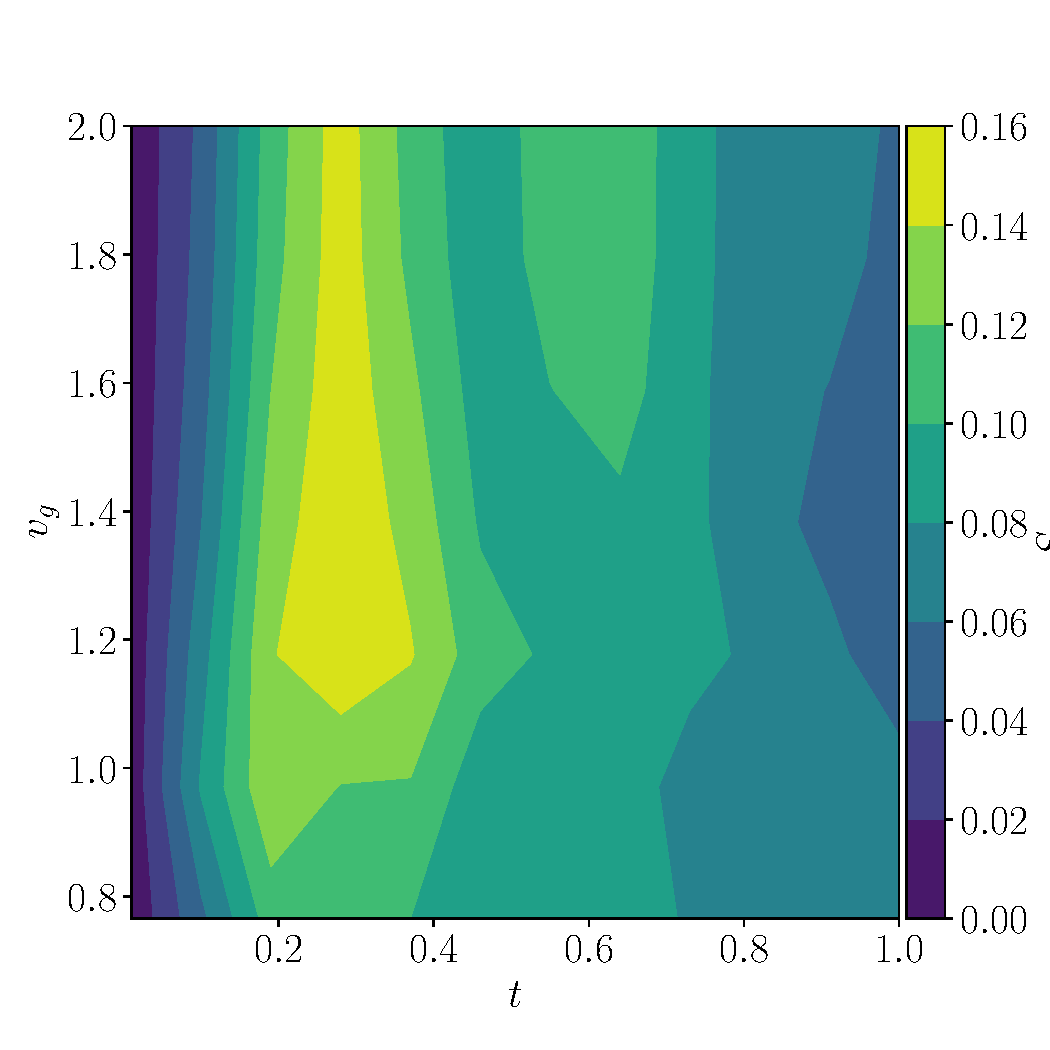
\includegraphics[width=\textwidth]{figures/report_04_2025/entropy_phase_diagram.pdf}
        \caption{}
    \end{subfigure}
    \vspace{0.001\textwidth}
    \begin{subfigure}[b]{0.85\textwidth}
        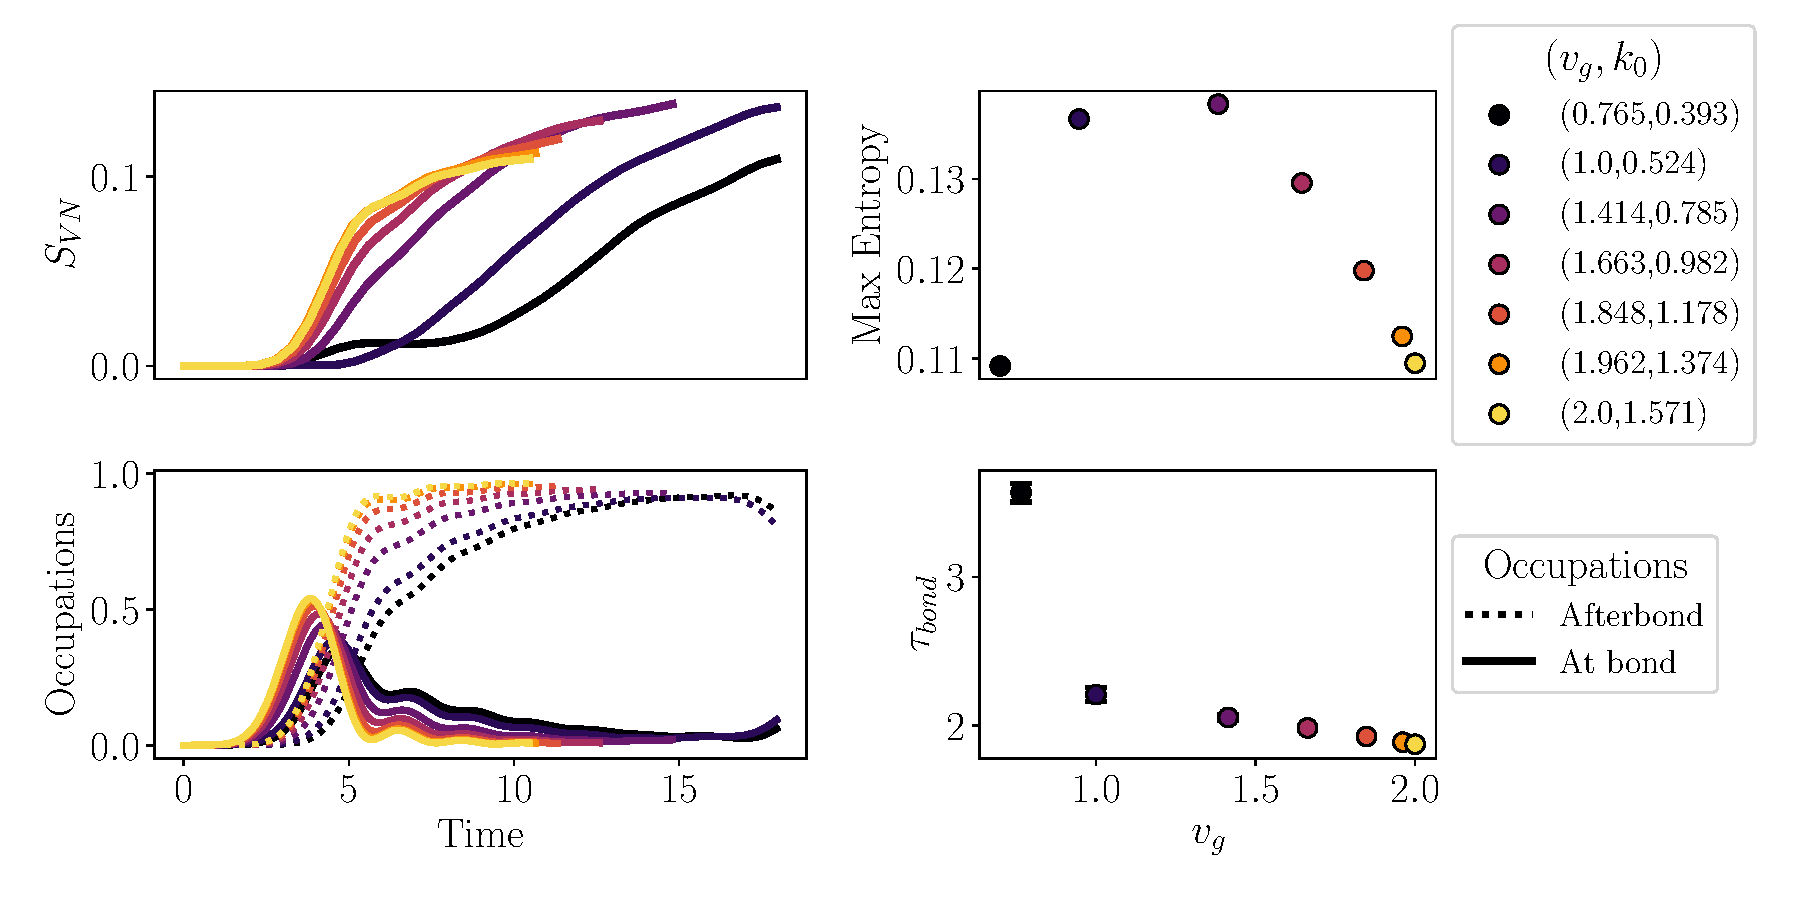
\includegraphics[width=\textwidth]{figures/report_04_2025/entropy_summary.pdf}
        \caption{}
    \end{subfigure}
    \caption{Generated von Neumann entropy ($S_{\rm V N}$) with $\Omega = 0.3$ as a function
            of group velocity $v_g$ and double dot hopping $t$. (a) Phase diagram for the entropy,
            shown in color (b) Unraveling of the phase diagram at $t=0.1$, showing the different
            velocities as different colors. The left column shows the entropy as a function of 
            time on top of the occupations to the left of the bond (dashed line) and at the 
            bond (solid). The right column shows the maximum entropy on 
            top of the time $\tau_{\rm bond}$ that the QPC particle spends at the bond. Both as a function
            of the group velocity and each point color coded to correspond to each group velocity.}
    \label{fig:entropy_phase_diagram}
\end{figure}

Finally, we can compare the predicted extra phase from the $\gamma$ obtained in section 
\ref{sect:bloch_backaction} with the numerical results. 
Figure \ref{fig:phase_backaction} shows $\gamma$ as a function $k_0$ for two different $\Omega$.
Despite the naive expectation from $\gamma := 2\Omega T k_0$ of a linear dependence,
as previous results indicate, the measurement time window is in itself dependent on $k_0$, 
hence the complex behavior. This figure also indicates that there is a large 
disagreement between analytics and numerics. While, the error is reduced at smaller $\Omega$ 
it is still significant. \sj{It is not clear whether this is an issue with the estimation 
of $T$ as the FWHM, or due to the approximations made in section \ref{sect:bloch_backaction}}. 

\begin{figure}[h]
    \centering
    \begin{subfigure}[b]{0.45\textwidth}
        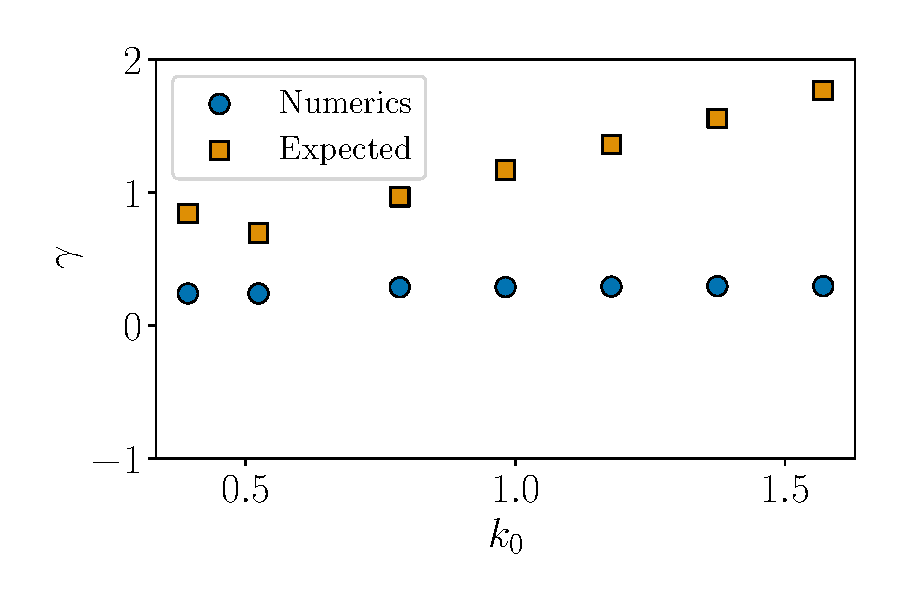
\includegraphics[width=\textwidth]{figures/report_04_2025/extra_phase_om=0.3.pdf}
        \caption{}
    \end{subfigure}
    \hspace{0.001\textwidth}
    \begin{subfigure}[b]{0.45\textwidth}
        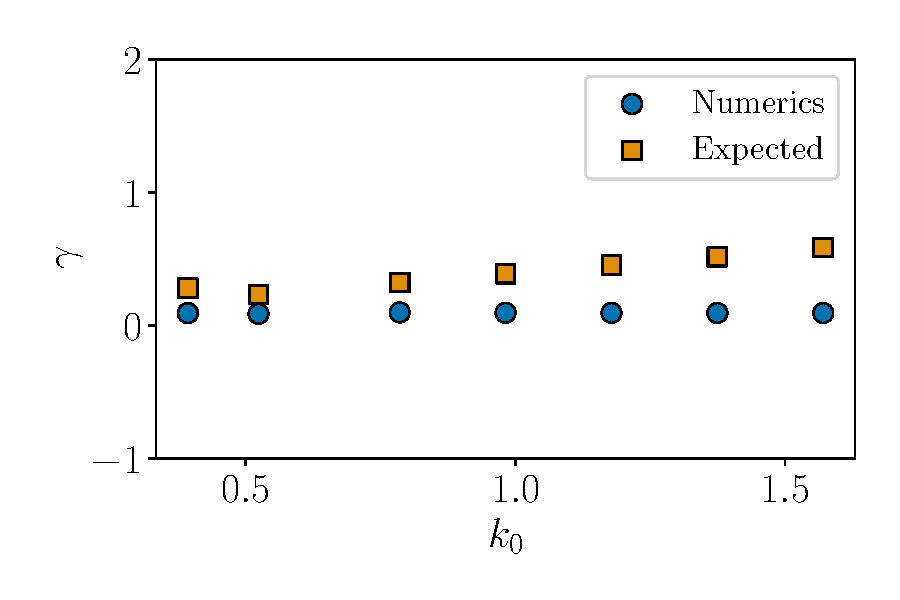
\includegraphics[width=\textwidth]{figures/report_04_2025/extra_phase_om=0.1.pdf}
        \caption{}
    \end{subfigure}
    \caption{Additional phase $\gamma$ induced on the double dot with $t=0.1$ due to
     the backaction of the QPC as a function of the central momentum. (a) Example with $\Omega=0.3$.
     (b) Example with $\Omega=0.1$. The measurement window $T$ has been estimated from 
     the FWHM of the bond density.}
    \label{fig:phase_backaction}
\end{figure}

\bibliography{qpc}
\bibliographystyle{ieeetr}



\end{document}